\documentclass[border=10pt]{standalone}
\usepackage[svgnames]{xcolor}
\usepackage{amsmath}
\usepackage{pgfplots}
\pgfplotsset{compat=newest}
\usepackage[sfdefault]{FiraSans}
\usepackage{FiraMono}
\renewcommand*\familydefault{\sfdefault}
\begin{document}
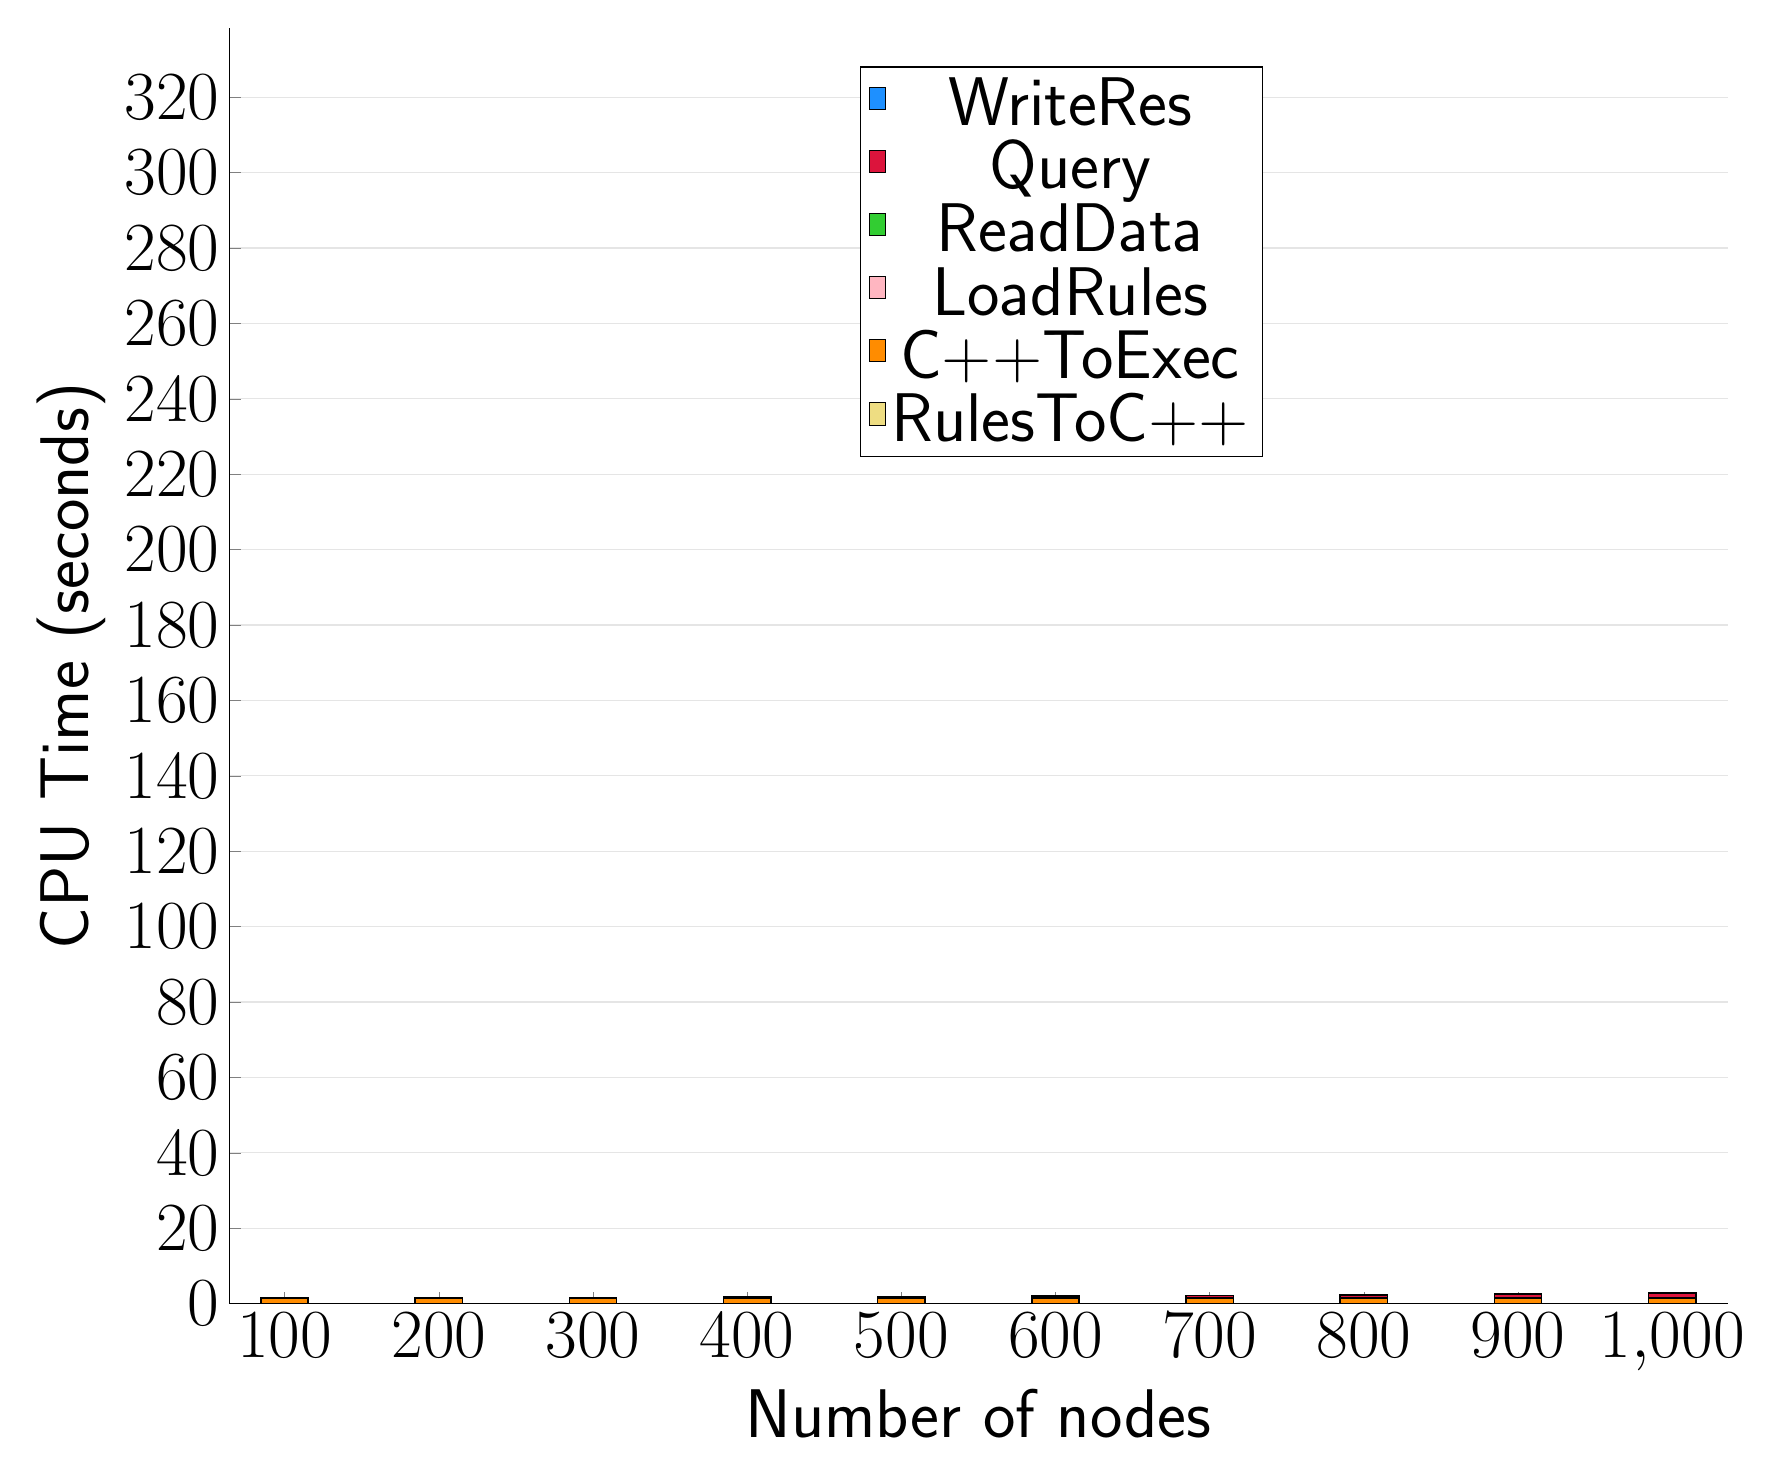
\begin{tikzpicture}
\begin{axis}[
   ybar stacked,
   width=1.7\textwidth,
   bar width=0.6cm,
   ymajorgrids, tick align=inside,
   major grid style={draw=gray!20},
   xtick=data,
   ymin=0, ymax=338.29920000000004,
   axis x line*=bottom,
   axis y line*=left,
   enlarge x limits=0.04,
   legend style={
       at={(0.69, 0.97)},
       anchor=north east,
       legend columns=1,
       font=\Huge,
   },
   ylabel={CPU Time (seconds)},
   xlabel={Number of nodes},
   label style={font=\Huge},
   tick label style={font=\Huge},
]
\addlegendimage{fill=DodgerBlue, draw=black, line width=0.2pt}
\addlegendentry{WriteRes}
\addlegendimage{fill=Crimson, draw=black, line width=0.2pt}
\addlegendentry{Query}
\addlegendimage{fill=LimeGreen, draw=black, line width=0.2pt}
\addlegendentry{ReadData}
\addlegendimage{fill=LightPink, draw=black, line width=0.2pt}
\addlegendentry{LoadRules}
\addlegendimage{fill=DarkOrange, draw=black, line width=0.2pt}
\addlegendentry{C++ToExec}
\addlegendimage{fill=LightGoldenrod, draw=black, line width=0.2pt}
\addlegendentry{RulesToC++}
\addplot +[fill=LightGoldenrod, draw=black, line width=0.55pt] coordinates {
(100, 0.0020000000000000005)
(200, 0.010000000000000002)
(300, 0.008000000000000002)
(400, 0.006000000000000001)
(500, 0.010000000000000002)
(600, 0.008000000000000002)
(700, 0.010000000000000002)
(800, 0.008000000000000002)
(900, 0.004000000000000001)
(1000, 0.006000000000000001)
};
\addplot +[fill=DarkOrange, draw=black, line width=0.55pt] coordinates {
(100, 1.53)
(200, 1.5260000000000002)
(300, 1.518)
(400, 1.5220000000000002)
(500, 1.52)
(600, 1.516)
(700, 1.512)
(800, 1.514)
(900, 1.5220000000000002)
(1000, 1.5079999999999998)
};
\addplot +[fill=LightPink, draw=black, line width=0.55pt] coordinates {
(100, 0.00015140000000000002)
(200, 0.0001574)
(300, 0.0001522)
(400, 0.0001498)
(500, 0.0001496)
(600, 0.00015040000000000002)
(700, 0.00014580000000000002)
(800, 0.00015219999999999999)
(900, 0.0001494)
(1000, 0.00012100000000000001)
};
\addplot +[fill=LimeGreen, draw=black, line width=0.55pt] coordinates {
(100, 0.0009195999999999999)
(200, 0.0012528)
(300, 0.0016649999999999998)
(400, 0.002018)
(500, 0.0024748)
(600, 0.0028404000000000003)
(700, 0.0031977999999999998)
(800, 0.00344)
(900, 0.0035796)
(1000, 0.0036471999999999997)
};
\addplot +[fill=Crimson, draw=black, line width=0.55pt] coordinates {
(100, 0.021382599999999998)
(200, 0.0631578)
(300, 0.12015419999999999)
(400, 0.20052280000000003)
(500, 0.30798739999999997)
(600, 0.4400102)
(700, 0.5994596)
(800, 0.7857758)
(900, 1.0054919999999998)
(1000, 1.2515199999999997)
};
\addplot +[fill=DodgerBlue, draw=black, line width=0.55pt] coordinates {
(100, 0.0002882)
(200, 0.0002394)
(300, 0.00023739999999999997)
(400, 0.0002606)
(500, 0.00029620000000000004)
(600, 0.00030680000000000003)
(700, 0.0003276)
(800, 0.0003302)
(900, 0.00032960000000000004)
(1000, 0.00035)
};
\end{axis}
\end{tikzpicture}

\end{document}
